\chapter{VS Code extension}

The frontend of the project is implented as an extension to a modern IDE, instead of creating a completely new GUI. This approach has the advantage of providing a familiar environment and workflow that the developers are used to.

There are several IDEs that currently (natively) support LSP, such as \emph{Eclipse Che} and \emph{Eclipse IDE}, \emph{vim8}, \emph{Visual Studio} and \emph{Visual Studio Code} and many more. Others, for example \emph{IntelliJ}, have plugins which add the support for LSP.

Our choice is \emph{Visual Studio Code}, due to its popularity and light-weight design. Conveniently, \emph{Theia}, a web-based IDE, supports VSCode extensions, therefore our plugin works with \emph{Theia} as well.

\section{Standard LSP Extension}

The core of the extension is an activation event which starts the plugin for VSCode.

On activation, \emph{Language Client} and \emph{Language server} are started as child processes of VSCode and a pipe is open for their communication. The LSP communication and its features are included in npm package \emph{vscodelc}. 

To be independent of pipes, we add an option to use TCP where a random free port is assigned for them to use.

\section{DAP Extension}

\emph{Macro Tracer}~(\autoref{chap:macro_tracer}) is implemented using DAP which is also supported out-of-the-box by VSCode. We dynamically set the random free port for DAP communication during activation.

\section{Additions}

Several features are added to the extension to improve the experience with HLASM and the extension as whole. These additions are specific for Visual Studio Code (and Theia) and are not part of the LSP specification.

\subsection{Language Detection}

The usual workflow with the extension begins with downloading HLASM source codes from Mainframe. Typically, these files won't have any file extension and if they do, they might differ across different products.

To cope with this problem, there are several mechanisms that recognize the file as HLASM.

\subsubsection{Macro Detection}

Each file starting with line \emph{MACRO} (arbirtary number of whitespace before and after) is recognized as HLASM.

\subsubsection{Configuration Files Detection}

Every file either defined as a program or a part of processor group is recognized as HLASM.

\subsubsection{Wildcards}

Configuration file \emph{pgm\_conf.json} contains field \emph{alwaysRecognize} which consists of user-defined wildcards. Every file that satisfies at least one of these wildcards is recognized as HLASM.

\subsubsection{Automatic Language Detection}

Whenever a file is open, it's contents are scanned line by line. Whether a file is HLASM or not is determined by a ratio (\# HLASM lines)/(\# all lines). A line is HLASM if:
\begin{enumerate}
	\item Line contains an instruction from a set of most used instructions and it is used correctly OR it is a continued line of correct HLASM line
	\item Line is not a comment (skipped otherwise)
	\item Line is not empty (skipped otherwise)
	\item Line is no longer than 80 characters
\end{enumerate}

We tested the detection on ~25.000 HLASM files. The best results were observed using ratio 4/10, with 88\% positive recognition and 95\% negative recognition (non-HLASM files not recognized as HLASM). 

Because of the uncertain outcomes, this method is meant to be used as a fall-back in case all previous methods do not suffice.

\subsection{Continuation Handling}

For historical reasons, HLASM has a 80 character per line limitation. Modern languages do not enforce such restriction and therefore IDEs such as VSCode allow the user to extend their lines freely. This causes 2 major inconveniences.

First of all, the user must add the continuation character on a very specific column manually. Secondly, each time the user types in between continuation character and the instruction/parameters, the continuation character moves from its requisite position and needs to be moved back, again manually.

To improve this behavior, the extension offers an option to activate \emph{Continuation Handling}. 

The first problem is solved by adding two editor commands \emph{insertContinuation} and \emph{deleteContinuation} which, when invoked, insert/delete the continuation character on its correct position.

To improve the second problem, the option overrides standard VSCode commands, commonly used when working in editor such as \emph{type}, \emph{deleteLeft}, \emph{deleteRight}, \emph{cut} and \emph{paste}. They offset the continuation character by removing/adding whitespaces in front of it.


\subsection{Configuration Prompt}

If the workspace contains HLASM file but it does not have configurations, the user is prompted to create them. This warning offers an option to create configuration templates.

\subsection{HLASM Semantic Highlighting}

In case of HLASM, a semantic (server-side) highlighting is desired. Multi-layered nature of the language causes that in quite common scenarios, specific parts of code can be highlighted if some previous part was completely processed (parameters for instructions, skipped code thanks to code generation, defined macros, continuations, etc...).

We added \emph{semanticHighlighting} as an extra feature of LSP. This feature works in a very similar manner, implementing the LSP interfaces that VSCode provides. It works as a notification from server to client, containing ranges of code and their respective tokens (e.g. instruction, label, parameter, comment,..).

On top of that, we extended \emph{semanticHighlighting} to \emph{ASMsemanticHighlighting}, which adds the ability to also notify the client of the new code layout, specifically start, continuation and continue columns. These fields can be set in HLASM code (via ICTL instruction) and are required for the \emph{Continuation Handling} feature to work properly. Our client-server communication is shown in \cref{fig08:lsp}.


\begin{figure}
	\centering
	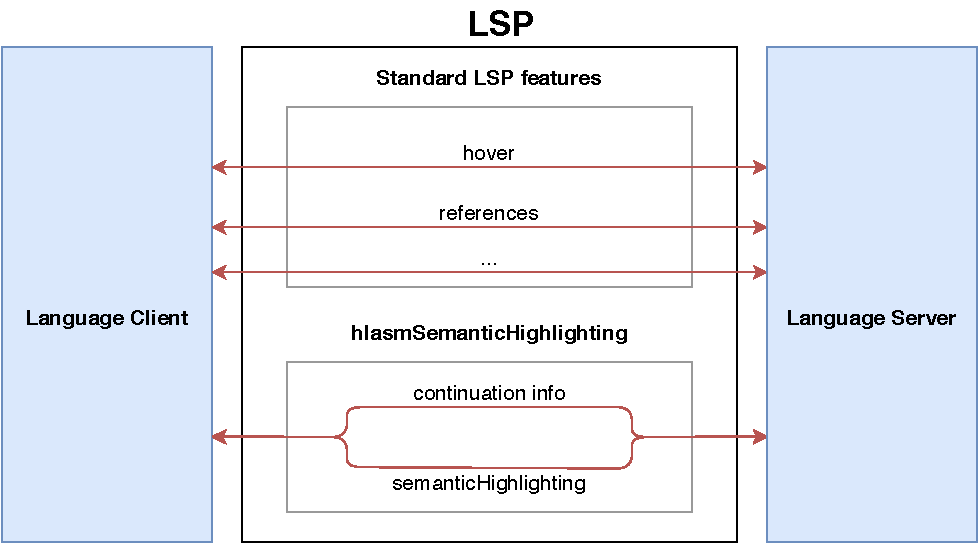
\includegraphics[width=\textwidth]{img/lsp_addition}
	\caption{The addition of semantic highlighting to the LSP communication.}
	
	\label{fig08:lsp}
\end{figure}

